\documentclass{beamer}
\usepackage{fontspec}
\usepackage[russian]{babel}
\usepackage{csquotes}
\usepackage{gost-table}
\usepackage{graphicx}
\graphicspath{{./images}}

%%% beamer
\setmainfont{Times New Roman}
\usefonttheme{serif}
\setbeamertemplate{frametitle}[default][center]
\usetheme{Singapore}
\addtobeamertemplate{navigation symbols}{}{%
    \usebeamerfont{footline}%
    \usebeamercolor[fg]{footline}%
    \hspace{1em}%
    \insertframenumber/\inserttotalframenumber
}
%%%

\begin{document}
\begin{frame}
    \begin{center}
        Липецкий государственный технический университет\\
        Кафедра автоматизированных систем управления
        \vfill
        ОТЧЕТ\\
        по преддипломной практике в ООО \textquote{Fusionsoft}\\
        по направлению 09.03.04 \textquote{Программная инженерия}\\
        \textquote{Разработка информационной системы поддержки технического
        обслуживания автомобильного парка}
    \end{center}
    \vfill
    \begin{tabularx}{\textwidth}{LR}
        Студент & Федин М.С. \\
        Группа ПИ-18 & \\
        Руководитель & \\
        к.т.н., доцент & Назаркин О.А.
    \end{tabularx}
\end{frame}

\begin{frame}
    {Характеристика объекта автоматизации или предметной области}
    В процессе эксплуатации автомобиля его составные части изнашиваются, что
    приводит к снижению эффективности или даже поломке.
    \\[\baselineskip]

    Существует два способа поддержания работоспособности автомобиля:
    \begin{itemize}
        \item техническое обслуживание (ТО);
        \item ремонт (Р).
    \end{itemize}
\end{frame}

\begin{frame}
	{Постановка задачи. Цели, критерии оценки и ограничения}
    Целью работы является автоматизация процессов учета и
    анализа деятельности организации, занимающейся обслуживанием
    автомобильной техники.
    \\[\baselineskip]

    Ключевые задачи, которые должна выполнять система:
    \begin{itemize}
        \item учет ресурсов, необходимых для проведения ТО;
        \item учет текущего состояния автомобилей;
        \item учет проведения сервисных работ;
        \item календарное планирование проведения ТО.
    \end{itemize}
\end{frame}

\begin{frame}
	{Основные понятия и процессы, их свойства и закономерности}
    Разрабатываемая информационная система должна обеспечивать выполнение
    следующих бизнес-процессов:
    \begin{itemize}
      \item обеспечивать просмотр и редактирование информации о конкретном
        автомобиле;
      \item обеспечивать просмотр и редактирование информации о текущем статусе
        работ;
      \item обеспечивать просмотр и редактирование информации о сотрудниках;

      \item составлять график прохождения технического обслуживания и ремонта
        техникой.
    \end{itemize}
\end{frame}

\begin{frame}
	{ER-диаграмма предметной области}
    \begin{figure}[h]
        \centering
        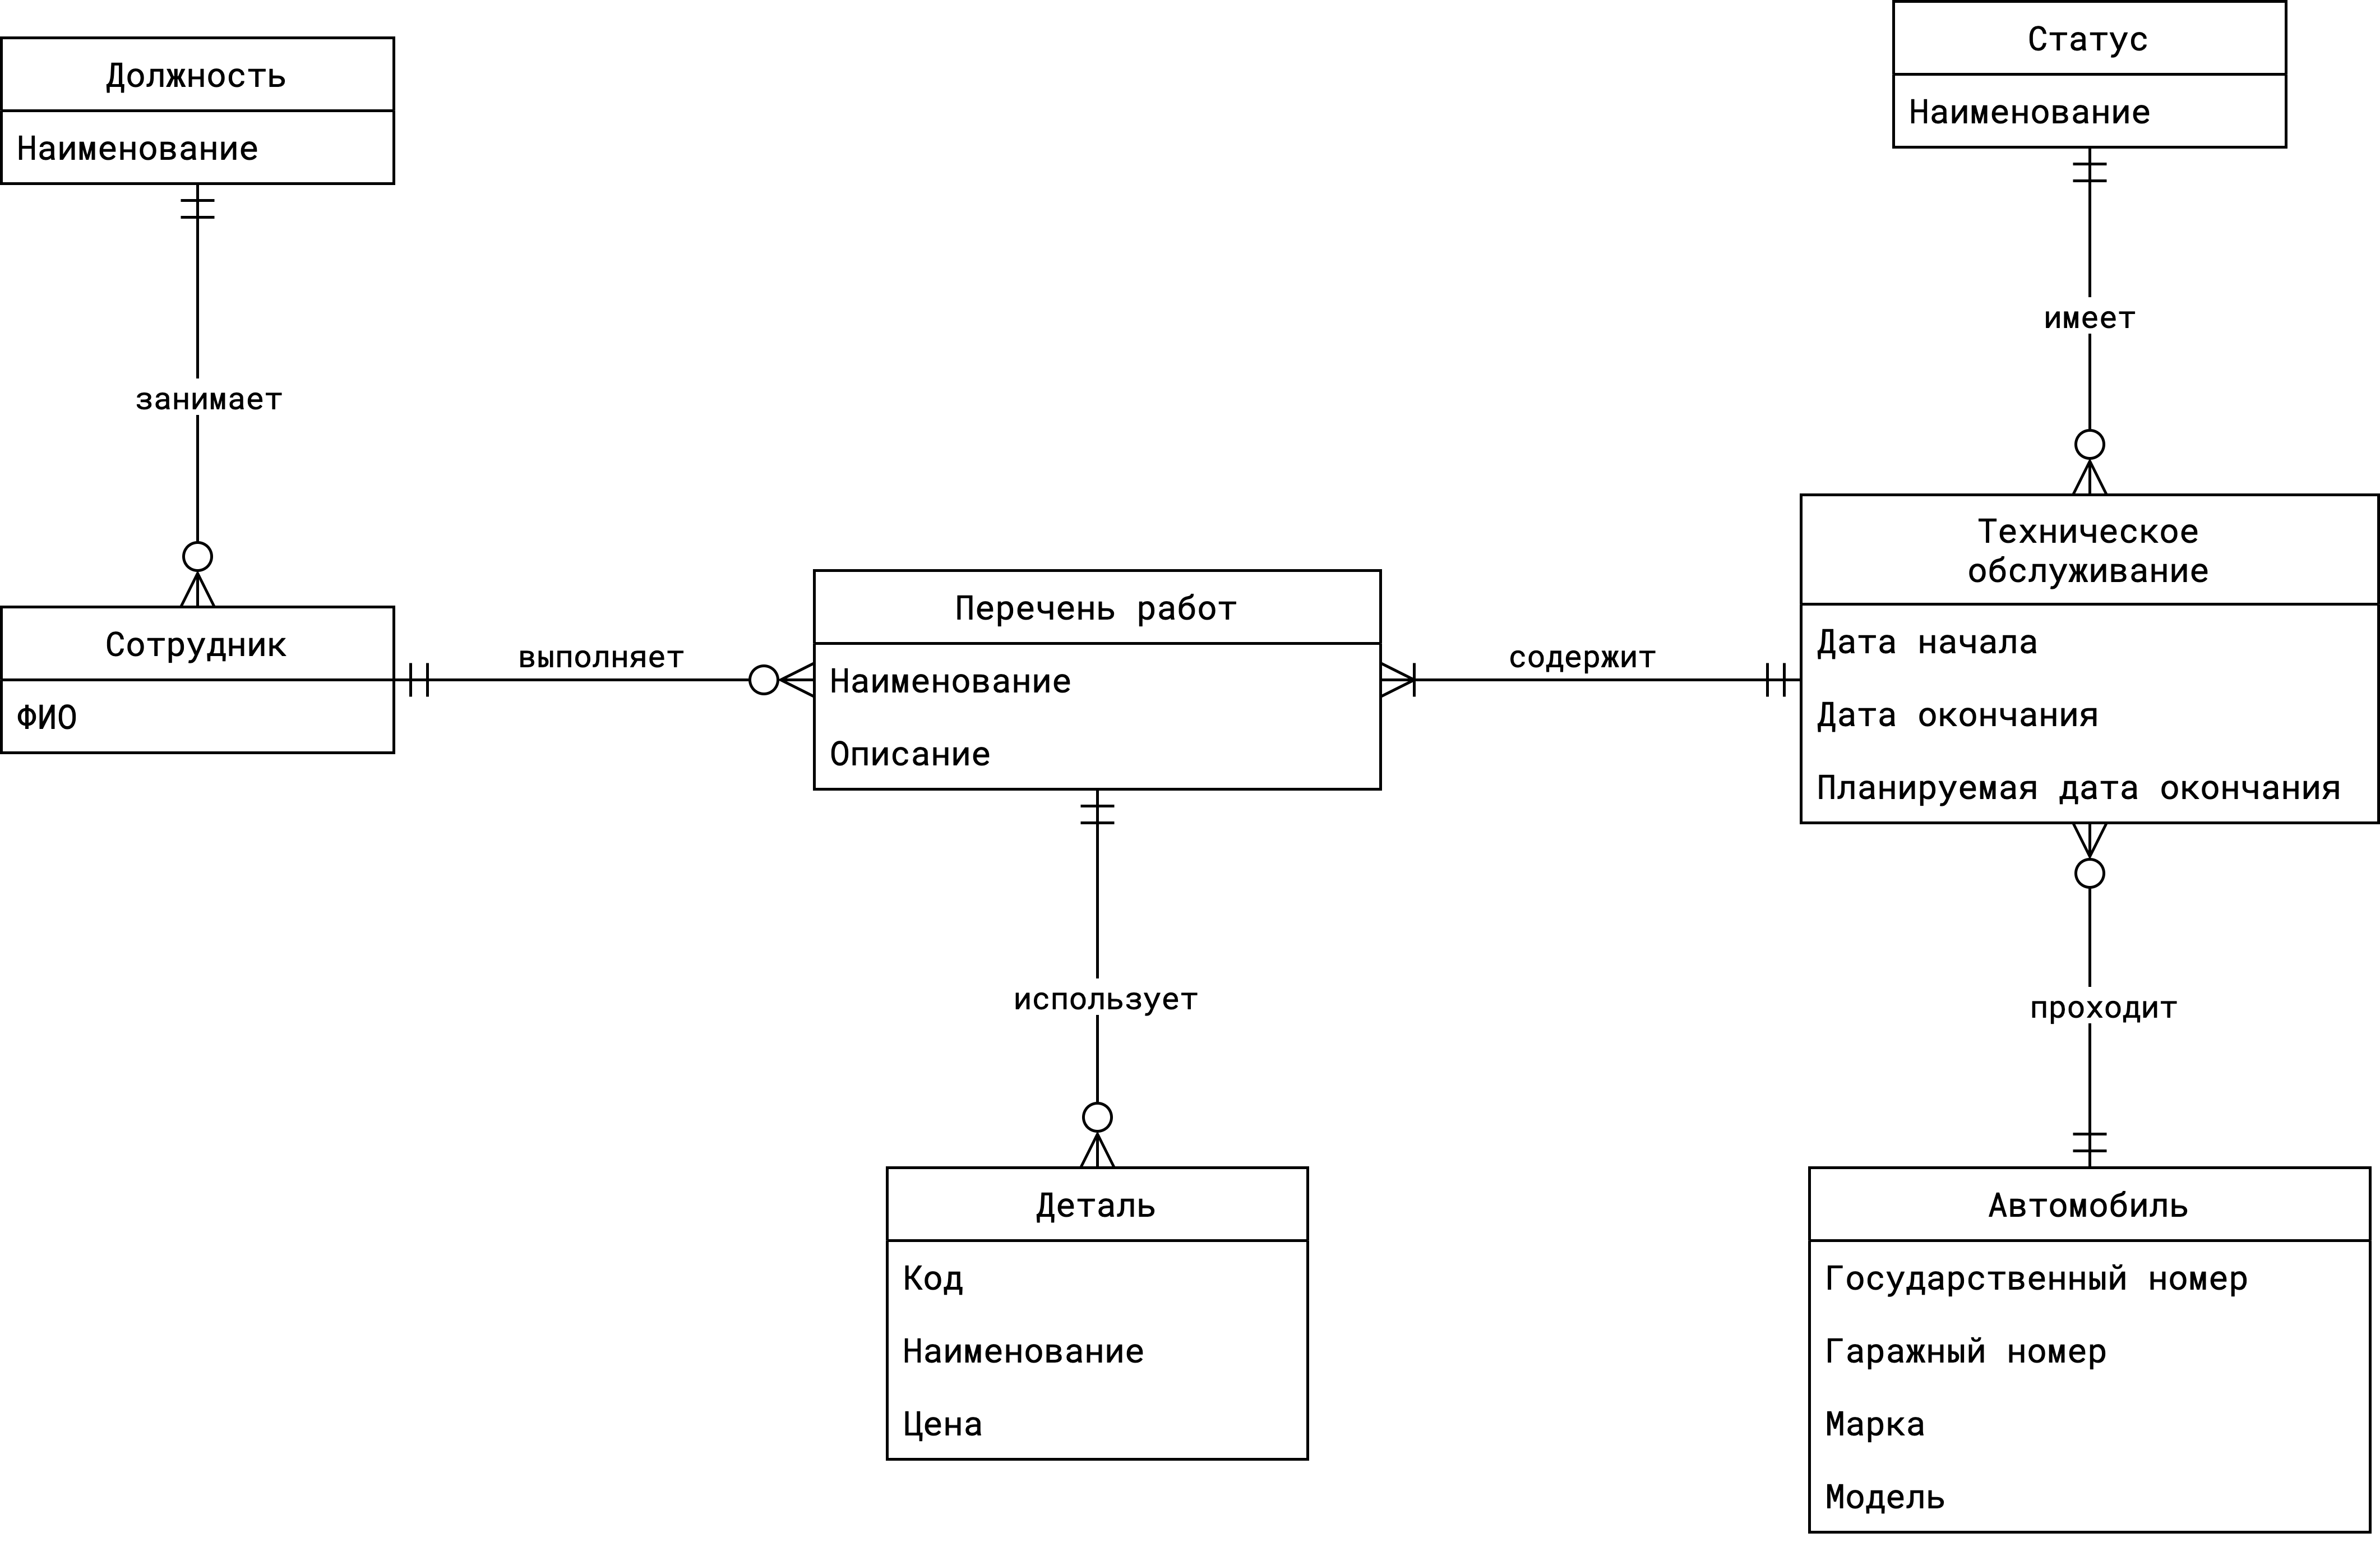
\includegraphics[keepaspectratio,width=\textwidth]{er-diagram.png}
        \label{fig:er-diagram}
    \end{figure}
\end{frame}

\begin{frame}
	{Теоретические математические модели}
\end{frame}

\begin{frame}
	{Эмпирические математические модели}
\end{frame}

\begin{frame}
	{Логическая модель данных}
\end{frame}

\begin{frame}
	{Физическая модель данных}
\end{frame}

\begin{frame}
	{Описание источников информации, входных сигналов и документов}
\end{frame}

\begin{frame}
	{Описание выходной информации: сигналов, документов и видеокадров}
\end{frame}
\end{document}
